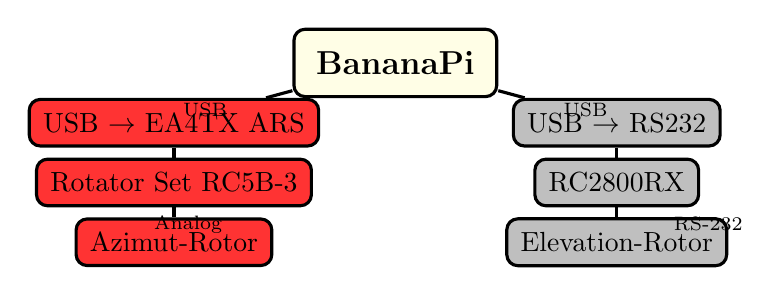
\begin{tikzpicture}[every node/.style = {shape=rectangle, rounded corners, draw, align=center, scale=1}, line width=0.4mm, level 
distance=1.8\baselineskip, level 1/.style = {sibling distance=16em}, level 2/.style = {sibling distance=8em}]
	\tikzstyle{top} = [fill=yellow!10, inner sep=8pt, font=\bfseries\large]
	\tikzstyle{az} = [fill=red!80, inner sep=5pt]
	\tikzstyle{el} = [fill=gray!50, inner sep=5pt]
	\tikzstyle{label} = [draw=none, font=\scriptsize, right]
	\node[top]{BananaPi}
	child { node[az]{USB $\rightarrow$ EA4TX ARS} 
		child { node[az]{Rotator Set RC5B-3} 
		  child { node[az]{Azimut-Rotor} } } }
	child { node[el]{USB $\rightarrow$ RS232}
		child { node[el]{RC2800RX}
		  child { node[el]{Elevation-Rotor} } } };
	\node[label] at (2,-0.6) {USB};
	\node[label,left] at (-2,-0.6) {USB};
	\node[label] at (-3.2,-2.05) {Analog};
	\node[label] at (3.4,-2.05) {RS-232};
% 	\node[label] at (-3.2,-3.5) {};
% 	\node[label] at (3.4,-3.5) {};
\end{tikzpicture} 
